\PassOptionsToPackage{usenames}{xcolor}
\PassOptionsToPackage{dvipsnames}{xcolor}
\documentclass[11pt,a4paper,twoside,final,titlepage,openright,fleqn]{book}%
\usepackage{beamerarticle}

\usepackage[utf8]{inputenc}
\usepackage[T1]{fontenc}
\usepackage[spanish]{babel}

\usepackage{listings}
\usepackage{palatino}
\usepackage{lmodern}

%\renewcommand*\rmdefault{lmr}
%\renewcommand*\ttdefault{ppl}

\usepackage{url}
\usepackage{multicol}

\usepackage{tabularx}

\usepackage{tikz}
\usetikzlibrary{positioning}
\usetikzlibrary{arrows}
\usetikzlibrary{mindmap}

\usepackage{pgfplots}
\pgfplotsset{compat=1.5}

\usepackage{ccicons}

\tikzset{
  invisible/.style={opacity=0},
  visible on/.style={alt=#1{}{invisible}},
  alt/.code args={<#1>#2#3}{%
    \alt<#1>{\pgfkeysalso{#2}}{\pgfkeysalso{#3}} % \pgfkeysalso doesn't change the path
  },
  bloque/.style={rectangle,draw=black, top color=white, bottom color=blue!50,
                 very thick, inner sep=0.5em, minimum size=0.6cm, text centered, font=\tiny},
  bloquelibre/.style={rectangle,draw=black, top color=white, bottom color=blue!10,
                 very thick, inner sep=0.5em, minimum size=0.6cm, text centered, font=\tiny},
  flecha/.style={->, >=latex', shorten >=1pt, thick},
  etiqueta/.style={text centered, font=\tiny} 
}



\usepackage[a4paper,left=2cm,right=2cm,top=2.5cm,bottom=4cm]{geometry}
\usepackage[colorlinks=true,linkcolor=blue,citecolor=blue,urlcolor=blue,plainpages=false,bookmarksnumbered=true,pdfpagemode=UseOutlines]{hyperref}


\usepackage[nottoc]{tocbibind}

%\usepackage[fixlanguage]{babelbib}


\usepackage{graphicx}
\usepackage{xcolor}
\usepackage{tikz}
\usetikzlibrary{arrows,positioning} 

\newcommand{\textgood}[1]{%
{\color{blue!60!black}\textbf{#1}}%
}

\newcommand{\textbad}[1]{%
{\color{red!80!black}\textbf{#1}}%
}

\newcommand{\textmark}[1]{%
{\color{orange!70!black}\textbf{#1}}%
}

\newcommand{\textenum}[1]{%
{\color{blue!60!black}\textbf{#1}}%
}

\newcommand{\textemph}[1]{%
{\color{green!40!black}\textbf{#1}}%
}

\newcommand{\versionid}{2021.1}
\newcommand{\versiondate}{Agosto de 2021}

\newcommand{\coursetitle}{Programación en C++ Vol. 2}
\newcommand{\modulenoexcept}{Especificaciones de excepciones}
\newcommand{\moduleconstrdestr}{Construcción y destrucción}
\newcommand{\modulecopia}{Mecanismos de copia}
\newcommand{\modulemove}{Operaciones de movimiento}
\newcommand{\modulememmgmt}{Gestión de memoria}

\newcommand{\pppbook}{\emph{Programming: Principles and Practice using C++, 2$^a$ edición~\cite{stroustrup:2014}}}
\newcommand{\cppbook}{\emph{The C++ Programming Language, 4$^a$ edición~\cite{stroustrup:2013}}}
\newcommand{\tourbook}{\emph{A tour of C++, 2$^a$ edición~\cite{stroustrup:2018}}}


\newtheorem{ejer}{Ejercicio}

\usepackage{url}

\usepackage{pdfpages}

\usepackage{todonotes}

%Package fancyhdr
\usepackage{fancyhdr}
\setlength{\headheight}{1.7cm}%{13.6pt}
\pagestyle{fancyplain}
\fancyhf{}
\lhead{
\includegraphics[height=1.25cm]{logos/uc3m.png}}
\chead{}
\rhead{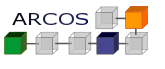
\includegraphics[height=1.25cm]{logos/arcos.png}}
\rfoot{\begin{tabular}{r}\coursetitle\\Versión \versionid\end{tabular}}
\cfoot{\begin{tabular}{c}{\thepage}\\{}\end{tabular}}
\lfoot{
\begin{tabular}{l}
\textbf{\ccbysa} -- CC BY-SA 4.0\\J. Daniel Garcia -- ARCOS@UC3M
\end{tabular}
}
\renewcommand{\headrulewidth}{0.5pt} % remove lines as well
\renewcommand{\footrulewidth}{0.5pt}
\renewcommand{\plainheadrulewidth}{0.5pt}
\renewcommand{\plainfootrulewidth}{0.5pt}

\renewcommand{\topfraction}{0.9}
\renewcommand{\textfraction}{0.1}
\renewcommand{\floatpagefraction}{0.9}

\usepackage{palatino}
\usepackage{lmodern}

\renewcommand*\rmdefault{lmr}
\renewcommand*\ttdefault{ppl}

\makeindex

\begin{document}

\mode<article>{
\lstset{
  language=C++,
  belowcaptionskip=1\baselineskip,
  breaklines=true,
  xleftmargin=\parindent,
  showstringspaces=false,
  basicstyle=\small,
  keywordstyle=\bfseries\color{green!40!black},
  commentstyle=\itshape\color{purple!40!black},
  identifierstyle=\color{blue},
  stringstyle=\color{brown},
  columns=fullflexible,
  inputencoding=utf8,
  extendedchars=true,
  upquote=true,
  morekeywords=[1]{_Pragma,constexpr,nullptr,alignof,alignas,decltype,override,final,noexcept,deprecated,thread_local,co_await,co_return,co_yield,fallthrough},
  literate=%
    {¿}{{?`}}{1}
    {¡}{{!`}}{1}
    {á}{{\'a}}{1}
    {é}{{\'e}}{1}
    {í}{{\'i}}{1}
    {ó}{{\'o}}{1}
    {ú}{{\'u}}{1}
    {ñ}{{\~n}}{1}
}
}

\mode<presentation>{
\lstset{
  language=C++,
  belowcaptionskip=1\baselineskip,
  breaklines=true,
  xleftmargin=\parindent,
  showstringspaces=false,
  basicstyle=\scriptsize,
  keywordstyle=\bfseries\color{green!40!black},
  commentstyle=\itshape\color{purple!40!black},
  identifierstyle=\color{blue},
  stringstyle=\color{orange},
  directivestyle=\bfseries\color{green!40!black},
  columns=fullflexible,
  inputencoding=utf8,
  extendedchars=true,
  upquote=true,
  morekeywords=[1]{_Pragma,constexpr,nullptr,alignof,alignas,decltype,override,final,noexcept,deprecated,thread_local,co_await,co_return,co_yield,fallthrough},
  literate=%
    {¿}{{?`}}{1}
    {¡}{{!`}}{1}
    {á}{{\'a}}{1}
    {é}{{\'e}}{1}
    {í}{{\'i}}{1}
    {ó}{{\'o}}{1}
    {ú}{{\'u}}{1}
    {ñ}{{\~n}}{1}
}
}

\newcommand{\cppkey}[1]{%
{\color{green!40!black}\textbf{#1}}%
}

\newcommand{\cppid}[1]{%
{\color{blue}\textbf{#1}}%
}

\newcommand{\cppstr}[1]{%
{\color{orange}\textbf{#1}}%
}


\lstdefinestyle{terminal}{
  language=bash,
  basicstyle=\scriptsize\ttfamily,
  numbersep=3pt,
  frame=tb,
  columns=fullflexible,
  backgroundcolor=\color{yellow!20},
}



\frontmatter

\pagestyle{empty}
\begin{titlepage}
\tikz[remember picture,overlay] \draw [fill,Blue] (current page.north west) rectangle +(0.2\paperwidth,-\paperheight);
\begin{flushright}

\includegraphics[width=5cm]{logos/uc3m.png}
\\
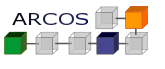
\includegraphics[width=5cm]{logos/arcos.png}
\end{flushright}

\vfill

\begin{tabular}{p{3cm}l}
&
\LARGE{Material de curso}
\\

&\\

&
\LARGE{\coursetitle}
\\

&\\

&
Version: \versionid
\\

&
\versiondate
\\

\end{tabular}
\vfill
\begin{tabular}{p{3cm}l}
&José Daniel García Sánchez\\
&Departamento de Informática\\
&Grupo ARCOS\\
&Universidad Carlos III de Madrid\\
&Av. Universidad, 30\\
&28911 Leganés, Madrid\\
&\url{josedaniel.garcia@uc3m.es}\\
\end{tabular}
\vspace{1cm}
\\
\begin{tabular}{p{3cm}l}
&
%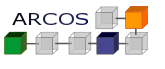
\includegraphics[width=5cm]{logos/arcos.png}
%\includegraphics[width=8cm]{logos/logo-uc3m.jpg}
\\
\end{tabular}
\end{titlepage}

\pagestyle{fancyplain}
\chapter*{Atribución-CompartirIgual 4.0 Internacional (CC BY-SA 4.0)}

Este es un resumen legible por humanos (y no un sustituto) de la
(código legal disponible en
\url{https://creativecommons.org/licenses/by-sa/4.0/legalcode}
).

\section*{Usted es libre de:}

\begin{itemize}

\item \textbf{Compartir} --
copiar y redistribuir el material en cualquier medio o formato.

\item \textbf{Adaptar} -- 
remezclar, transformar y construir a partir del material
para cualquier propósito, incluso comercialmente.

\end{itemize}

La licenciante no puede revocar estas libertades en tanto usted siga los
términos de la licencia.

\section*{Bajo los siguientes términos:}

\begin{itemize}

\item \ccAttribution \quad \textbf{Atribución} --
Usted debe dar crédito de manera adecuada, brindar un enlace a la licencia, e
indicar si se han realizado cambios. Puede hacerlo en cualquier forma
razonable, pero no de forma tal que sugiera que usted o su uso tienen el apoyo
de la licenciante. 

\item \ccShareAlike \quad \textbf{CompartirIgual} --
Si remezcla, transforma o crea a partir del material, debe distribuir su
contribución bajo la lamisma licencia del original. 

\item \textbf{No hay restricciones adicionales} -- 
No puede aplicar términos legales ni medidas tecnológicas que restrinjan
legalmente a otras a hacer cualquier uso permitido por la licencia. 

\end{itemize}

\section*{Avisos:}

No tiene que cumplir con la licencia para elementos del materiale en el dominio
público o cuando su uso esté permitido por una excepción o limitación
aplicable.

No se dan garantías. La licencia podría no darle todos los permisos que
necesita para el uso que tenga previsto. Por ejemplo, otros derechos como
publicidad, privacidad, o derechos morales pueden limitar la forma en que
utilice el material.


\cleardoublepage
\chapter*{Presentación}

Bienvenidos al Volumen 2 del curso de C++.


\section*{Structure}

Los contenidos de este curso se estructuran de la siguiente forma:

\begin{enumerate}

\item \ldots

\end{enumerate}

\cleardoublepage
\chapter*{Agradecimientos}

En primer lugar, me gustaría dar las gracias a Bjarne Stroustrup
por darnos el lenguaje de programación C++.

También me gustaría expresar mi gratitud a todos los miembreos del
grupo de trabajo ISO/IEC JTC1/SC22/WG21, que han trabajado durante
décadas para mejorar y actualizar el lenguaje.
La discusión con muchos de ellos sobre diversos aspectos específicos
del lenguaje y de la biblioteca estándar han sido para mi de gran utilidad.

Así mismo, me gustaría agradecer de forma especial a todos aquellos
que han proporcionado realimentación sobre versiones previas de este 
material.


\cleardoublepage
\tableofcontents
\todototoc
\listoftodos

\mainmatter

\pagestyle{fancyplain}
\mode<article>{\chapter{\moduleconstrdestr}}

\mode<presentation>{\begin{frame}[shrink=20]{Licencia Creative Commons}

\begin{tabularx}{.98\textwidth}{lX}
\ccLogo & Este trabajo se distribuye bajo licencia
Atribución-NoComercial-SinDerivadas 4.0 Internacional (CC BY-NC-ND 4.0).\\

&\\

& \multicolumn{1}{c}{\textbf{Usted es libre de}:}\\

&\\

&
\textbf{Compartir} --
copiar y redistribuir el material en cualquier medio o formato.
\\

&\\

& \multicolumn{1}{c}{\textbf{Bajo los siguientes términos}:}\\

&\\

\ccAttribution &
Atribución -- Usted debe dar crédito de manera adecuada, brindar un enlace a la licencia, e indicar si se han realizado cambios. Puede hacerlo en cualquier forma razonable, pero no de forma tal que sugiera que usted o su uso tienen el apoyo de la licenciante.
\\

\ccNonCommercialEU &
NoComercial -- Usted no puede hacer uso del material con propósitos comerciales. 
\\

\ccNoDerivatives &
SinDerivadas -- Si remezcla, transforma o crea a partir del material, no podrá distribuir el material modificado. 
\\

\end{tabularx}

\end{frame}
}
\section{Desarrollo de un vector numérico}

\begin{frame}[t,fragile]{Objetivo}
\begin{itemize}
\item En esta unidad iremos incorporando los conceptos al desarrollo de un tipo 
      \textmark{vector numérico}: \cppid{vecnum}.
  \begin{itemize}
    \item Tipo con funcionalidad parecidad a \cppid{vector<double>}.
  \end{itemize}
\begin{lstlisting}
  vecnum v(5);
  v[2] = 3.0;
  for (int i=0; i<v.tamanyo(); ++i) {
    std::cout << "v[" << i << "] = " << v[i] << '\n';
  }
\end{lstlisting}

  \mode<presentation>{\vfill\pause}
  \item \textgood{Alternativas}:
  \begin{itemize}
    \item Usando \cppid{unique\_ptr}.
    \item Usando punteros primitivos.
  \end{itemize}

\end{itemize}
\end{frame}

\begin{frame}[t]{Usando \textbf{unique\_ptr}}
\begin{block}{vecnum.hpp}
\lstinputlisting[basicstyle=\tiny]{ejemplos/01-constr-destr/smart-vecnum/vecnum.hpp}
\end{block}
\end{frame}

\begin{frame}[t]{Usando \emph{punteros primitivos}}
\begin{block}{vecnum.hpp}
\lstinputlisting[basicstyle=\tiny]{ejemplos/01-constr-destr/primitive-vecnum/vecnum.hpp}
\end{block}
\end{frame}


\begin{frame}[fragile]{Comprobación de memoria}
\begin{itemize}
  \item \textgood{valgrind}: 
        Conjunto de herramientas para realizar análisis dinámico de programas.
    \begin{itemize}
      \item \textmark{memcheck}: Herramienta para:
        \begin{itemize}
          \item Accesos indebidos a memoria.
          \item Usos peligrosos de valores no iniciados.
          \item Goteos de memoria.
          \item Errores en liberación de memoria.
        \end{itemize}
    \end{itemize}
  \item Invocación:
\begin{lstlisting}[style=terminal]
valgrind --tool=memcheck programa
\end{lstlisting}
\begin{lstlisting}[style=terminal]
...
==15344== HEAP SUMMARY:
==15344==     in use at exit: 40 bytes in 1 blocks
==15344==   total heap usage: 1 allocs, 0 frees, 40 bytes allocated
==15344== LEAK SUMMARY:
==15344==    definitely lost: 40 bytes in 1 blocks
...
\end{lstlisting}
\end{itemize}
\end{frame}

\begin{frame}[t]{\textbf{valgrind} desde CLion}
\begin{itemize}
  \item \textmark{valgrind} está integrado en \textmark{CLion}.
    \begin{itemize}
      \item Se puede ejecutar desde \textgood{Run} | \textgood{Rin with valgrind memcheck}.
      
\includegraphics[width=2em]{images/01-constr-destr/valgrind.png}
    \end{itemize}
  \mode<presentation>{\vfill\pause}
  \item Resultado en panel de \textmark{Run valgrind memcheck}.
\end{itemize}
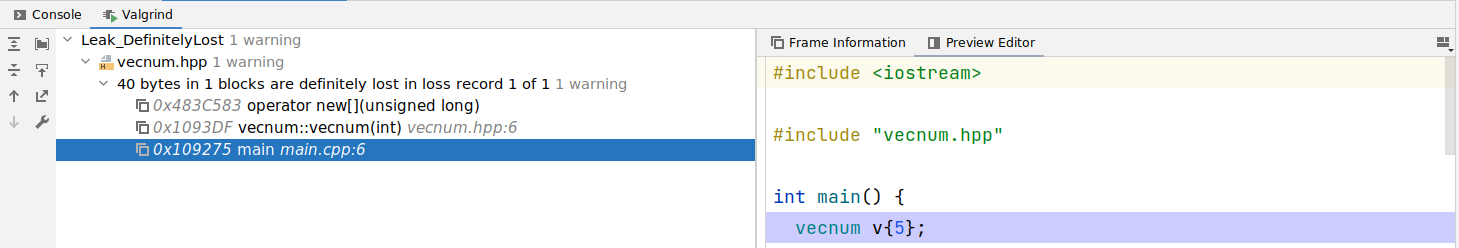
\includegraphics[width=\textwidth]{images/01-constr-destr/vecnum-main-valgrind.png}
\mode<presentation>{\vfill\pause}
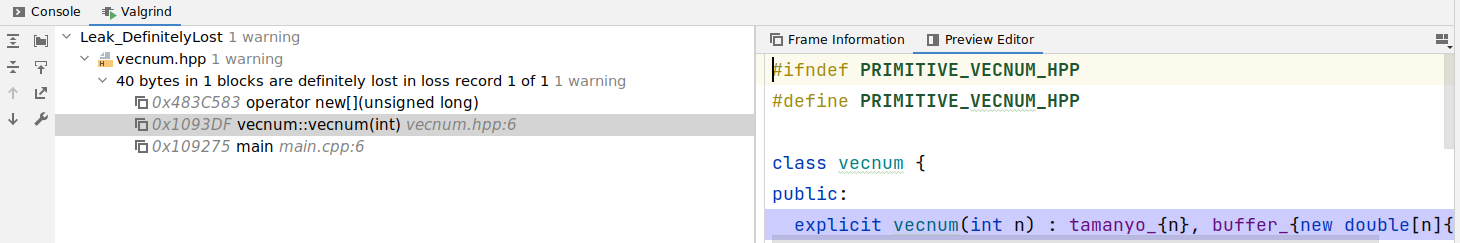
\includegraphics[width=\textwidth]{images/01-constr-destr/vecnum-ctor-valgrind.png}
\end{frame}

\begin{frame}[t]{Otra alternativa: \emph{sanitizers}}
\begin{itemize}
  \item Un \textgood{sanitizer} es una opción que instrumenta el código generado
        para detectar distintos tipos de errores.
    \begin{itemize}
      \item \textmark{AddressSanitizer}: Detecta errores de memoria.
      \item \textmark{LeakSanitizer}: Subconjunto de AddressSanitizer para goteos de memoria.
      \item \textmark{ThreadSanitizer}: Detecta errores de concurrencia.
      \item \textmark{UndefinedBehaviorSanitizer}: Detecta comportamientos no definidos.
      \item \textmark{MemorySanitizer}: Detecta acceso a memoria no iniciada (solo \textgood{clang}).
    \end{itemize}
\end{itemize}
\end{frame}

\begin{frame}[t,fragile]{Uso de \textbf{AddressSanitizer}}
\begin{itemize}
  \item Modificación de opciones de compilación y enlace.
\end{itemize}
\begin{lstlisting}
add_compile_options(-fsanitize=address)
add_link_options(-fsanitize=address)
\end{lstlisting}
\mode<presentation>{\vfill\pause}
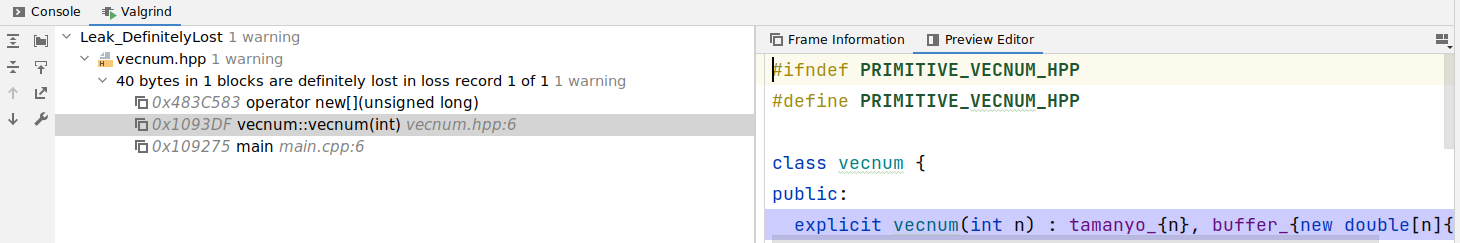
\includegraphics[width=\textwidth]{images/01-constr-destr/vecnum-ctor-valgrind.png}
\mode<presentation>{\vfill\pause}

\begin{columns}[T]
\column{.5\textwidth}
\textgood{AddressSanitizer}
{\mode<presentation>{\footnotesize}
\begin{itemize}
  \item Instrumentación binaria
  \item Deceleración = 2x
  \item Detecta desbordamientos
  \item No detecta accesos a memoria sin iniciar
\end{itemize}
}

\column{.5\textwidth}
\textgood{valgrind memcheck}
{\mode<presentation>{\footnotesize}
\begin{itemize}
  \item Instrumentación en compilación
  \item Deceleración = 20x
  \item No detecta desbordamientos
  \item Detecta accesos a memoria sin iniciar
\end{itemize}
}

\end{columns}
\end{frame}

\section{Destructores}

\begin{frame}[fragile]{El problema de la desasignación}
\begin{itemize}
  \item Un tipo que adquiere \textmark{recursos} (ej. memoria) 
        y no lo libera provoca un \textbad{goteo de memoria}.

  \mode<presentation>{\vfill\pause}
  \item \textgood{Solución simple}:
    \begin{itemize}
      \item Función miembro de liberación.
    \end{itemize}
\begin{lstlisting}
class vecnum {
  // ...
  void libera() { delete []v; }
  // ...
};

void f() {
  vecnum v{5};
  // ...
  otra_funcion(); // <- ¿Y si lanza una excepción?
  // ...
  v.libera(); // Fácil de olvidar
}
\end{lstlisting}
\end{itemize}
\end{frame}

\begin{frame}[fragile]{Función miembro de destrucción}
\begin{itemize}
  \item Un \textgood{destructor} es una función miembro especial que se ejecuta 
        \textmark{de forma automática} cuando un objeto sale de alcance.
    \begin{itemize}
      \item No tiene tipo de retorno.
      \item No toma parámetros.
      \item Su nombre es el nombre de clase precedido del símbolo \cppkey{\~}.
    \end{itemize}

\mode<presentation>{\vfill\pause}
\begin{lstlisting}
class vector {
  // ...
  ~vector() { delete []v; }
  // ...
};
\end{lstlisting}

  \mode<presentation>{\vfill\pause}
  \item Invocación automática.
\begin{lstlisting}
void f() {
  vecnum v{5};
  // ...
  otra_funcion(); // Si lanza excepción -> v se destruye
  // ...
} // v se destruye al salir
\end{lstlisting}
\end{itemize}
\end{frame}

\begin{frame}[fragile]{Destrucción generada por defecto}
\begin{itemize}
  \item En realidad \textmark{todos los tipos} tienen una función miembro 
        \textgood{destructor}.
    \begin{itemize}
      \item El \textmark{compilador genera automáticamente} una definición 
            que es \textgood{válida} en la mayoría de los casos.
    \end{itemize}

  \mode<presentation>{\vfill\pause}
  \item Dado un tipo \textbad{sin destructor}, 
        el compilador \textgood{sintetiza} uno que:
    \begin{itemize}
      \item Invoca (recursivamente) al destructor de cada miembro.
      \item El destructor de un tipo primitivo es la operación nula.
    \end{itemize}
\end{itemize}

\mode<presentation>{\vfill\pause}
\begin{lstlisting}
struct estudiante {
  string nombre;
  vector<double> notas;
  // ...
};

void f() {
  estudiante e { "Carlos", {9.0, 9.5, 8.5} };
  cout << e.nombre << " -> " << e.notas[0] << endl;
} // Destrucción de e -> Destrucción de e.nombre y e.notas
\end{lstlisting}
\end{frame}

\begin{frame}[t]{Vector numérico con destructor}
\begin{block}{vecnum.hpp}
\mode<presentation>{
  \lstinputlisting[basicstyle=\tiny]{ejemplos/01-constr-destr/primitive-vecnum-destr/vecnum.hpp}
}
\mode<article>{
  \lstinputlisting{ejemplos/01-constr-destr/primitive-vecnum-destr/vecnum.hpp}
}
\end{block}
\end{frame}

\section{Constructores}

\subsection{Tipos sin constructor}

\begin{frame}[t,fragile]{Iniciación sin constructor}
\mode<presentation>{\vspace{-1em}}
\begin{itemize}
  \item Iniciación de tipos primitivos.
\begin{lstlisting}
int x{1024}; // int x = 1024
double * p{nullptr}; // double * p = nullptr
\end{lstlisting}

  \mode<presentation>{\vfill\pause}
  \item Clases sin miembros privados que no tienen constructor:
\begin{lstlisting}
struct dispositivo {
  string id_serie;
  long long capacidad;
};
\end{lstlisting}

    \mode<presentation>{\vfill\pause}
    \begin{itemize}
      \item Iniciación por miembros:
\begin{lstlisting}
dispositivo d1{"hda1", 1024};
\end{lstlisting}

      \mode<presentation>{\vfill\pause}
      \item Iniciación directa
\begin{lstlisting}
dispositivo d3{d1}; // Copia miembro a miembro
\end{lstlisting}

      \mode<presentation>{\vfill\pause}
      \item Iniciación por defecto
\begin{lstlisting}
dispositivo d4{};
dispositivo d5;
\end{lstlisting}
    \end{itemize}
\end{itemize}
\end{frame}

\begin{frame}[t,fragile]{Iniciación por defecto}
\begin{itemize}
    \item Iniciación de \textgood{variables globales} $\Rightarrow$ 
          iniciación por defecto de \textmark{todos} los miembros.
\begin{lstlisting}
dispositivo d1; // id_serie="", capacidad=0
dispositivo d2{}; // id_serie="", capaciad=0
\end{lstlisting}

    \mode<presentation>{\vfill\pause}
    \item Iniciación de \textgood{variables locales} $\Rightarrow$ 
          iniciación por defecto \textmark{sólo} de miembros de tipo clase.
        \begin{itemize}
          \item Miembros de tipos primitivos \textbad{sin iniciar}.
        \end{itemize}
\begin{lstlisting}
void f() {
  dispositivo d3; // id_serie="", capacidad=?
  dispositivo d4{}; // id_sere="", capacidad=0
}
\end{lstlisting}
\end{itemize}
\end{frame}

\begin{frame}[t,fragile]{Iniciación de miembros por defecto}
\begin{itemize}  
  \item Se puede indicar valor por defecto para miembros.
\begin{lstlisting}
struct dispositivo {
  string id_serie{"sda1"};
  long long capacidad = 1024; // Notación alternativa
};

dispositivo d; // d.serie=="sda1", d.capacidad==1024
dispositivo e{"sda9"}; // e.serie="sda9", e.capacidad=1024
dispositivo f{2048}; // No compila
\end{lstlisting}

  \mode<presentation>{\vfill\pause}
  \item \textbad{Nota}: También conocida como \textmark{NSDMI}
        (non static data member initializers).
\end{itemize}
\end{frame}

\subsection{Tipos con constructor}

\begin{frame}[fragile]{Invocación al constructor}
\begin{itemize}
  \item Sin un tipo tiene uno o más constructores, 
        todas las definiciones de objetos \textgood{deben invocar} 
        \textmark{algún constructor}.
    \begin{itemize}
      \item El compilador \textbad{deja de generar} un 
            \textmark{constructor por defecto}.
    \end{itemize}
\begin{lstlisting}
struct complejo {
  double real, imag;
  complejo(double r);
  complejo(double r, double i);
};

complejo c1; // Error -> Sin constructor por defecto
complejo c2{}; // Error -> Sin constructor por defecto
complejo c3{2.0}; // OK
complejo c4{2.0, 3.5}; // OK
complejo * pc = new complejo{2.0,3.5}; // OK
complejo v[] { {1.0,1.5}, {2.0, 2.0} }; // OK
vector<complejo> w { {1.0, 1.5}, {2.0, 2.0} }; // OK
\end{lstlisting}
\end{itemize}
\end{frame}

\begin{frame}[fragile]{Invocación forzosa de constructor}
\begin{itemize}
  \item Existe una sintaxis para forzar la invocación de un constructor:
        \textmark{uso de paréntesis}.
    \begin{itemize}
      \item No invoca iniciación miembro a miembro o basadas en listas.
    \end{itemize}

\mode<presentation>{\vfill\pause}
\begin{lstlisting}
struct punto {
  double x, y;
};
punto p1(1.0, 1.0); // Error: No hay constructor
punto p2{1.0, 1.0}; // OK
punto p3(1.0); // Error: No hay constructor
punto p4{1.0}; // x=1.0, y=0.0
complejo c1(1.0, 1.0); // OK
complejo c2{1.0, 1.0}; // OK
complejo c3(1.0); // OK
complejo c4{1.0}; // OK
\end{lstlisting}

  \mode<presentation>{\vfill\pause}
  \item Útil para discriminar entre constructores de \cppid{std::vector} de tipos numéricos.
\begin{lstlisting}
vector<int> v{10}; // Vector con el valor 10. v.size() == 1
vector<int> v(10); // Vector con 10 valores 0. v.size() == 10
\end{lstlisting}
\end{itemize}
\end{frame}

\subsection{Constructor por defecto}

\begin{frame}[t,fragile]{Constructor por defecto}
\begin{itemize}
  \item El \textgood{constructor vacío} o \textmark{constructor por defecto} 
        es un constructor que no toma ningún parámetro.
\begin{lstlisting}
vector();
\end{lstlisting}

  \mode<presentation>{\vfill\pause}
  \item Define que debe hacerse:
    \begin{itemize}
      \item Cuando se \textmark{define un objeto} sin valor inicial.
\begin{lstlisting}
vector v;
vector v{};
\end{lstlisting}

      \mode<presentation>{\pause}
      \item Cuando se \textmark{asigna memoria} sin valor inicial
\begin{lstlisting}
vector * pv = new vector;
\end{lstlisting}

    \end{itemize}
\end{itemize}
\end{frame}

\begin{frame}[t,fragile]{Generación del constructor por defecto}
\mode<presentation>{\vspace{-.5em}}
\begin{itemize}
  \item El \textgood{constructor por defecto} se genera 
        \textbad{si no hay ningún constructor}.

\mode<presentation>{\vspace{-.75em}}
\begin{columns}[T]
\column{.2\textwidth}
\column{.5\textwidth}
\begin{lstlisting}
class vector {
public:
  //...
  //...
};
vector v; // OK
\end{lstlisting}

\column{.5\textwidth}
\begin{lstlisting}
class vector {
public:
  vector(int n);
  //...
};
vector v; // Error
\end{lstlisting}

\end{columns}

\mode<presentation>{\vfill\pause}
\item Se puede \textbad{forzar} la generación del \textgood{constructor por defecto} o
      \textbad{inhibir} su generación.

\mode<presentation>{\vspace{-.75em}}
\begin{columns}[T]
\column{.2\textwidth}
\column{.5\textwidth}
\begin{lstlisting}
class vector {
public:
  vector() = default;
  vector(int n);
  //...
};
vector v; // OK
\end{lstlisting}

\column{.5\textwidth}
\begin{lstlisting}
class vector {
public:
  vector() = delete;
  //...
  //...
};
vector v; // Error
\end{lstlisting}

\end{columns}

\end{itemize}
\end{frame}

\begin{frame}[t,fragile]{Constructor por defecto y arrays}
\begin{itemize}
  \item El tipo base de un array debe tener \textgood{constructor por defecto}, 
        sólo si hace falta iniciar por defecto.
\begin{lstlisting}
struct punto {
  double x, y;
  punto();
};
struct complejo {
  double real, imag;
  complejo(double d, double i);
};

std::array<punto,16> v; // OK
std::array<complejo,16> w; // Error: No pueden iniciarse elementos
std::array<complejo,2> c { {1.0, 1.0}, {2.0, 2.0} }; // OK 
\end{lstlisting}
\end{itemize}
\end{frame}

\begin{frame}[t,fragile]{Constructor por defecto y vectores}
\begin{itemize}
  \item El tipo base de un vector debe tener \textgood{constructor por defecto}, 
        si hace falta iniciar por defecto.
\begin{lstlisting}
struct punto {
  double x, y;
  punto();
};
struct complejo {
  double real, imag;
  complejo(double d, double i);
};

vector<punto> vp1; // OK. No necesita iniciar
vector<complejo> vc1; // OK. No necesita iniciar

vector<punto> vp2(16); // OK. 16 elementos con valor por defecto
vector<complejo> vc2(16); // Error: no puede iniciar 16 elementos
vector<complejo> vc3{ {1.0, 1.0}, {2.0, 2.0} }; // OK
vector<complejo> vc4{5, {1.0,1.0}}; // OK: 5 elementos iniciados
\end{lstlisting}
\end{itemize}
\end{frame}

\subsection{Conversión y constructor explícito}

\begin{frame}[fragile]{Constructor explícito}
\begin{itemize}
  \item Un constructor que recibe un único argumento define una 
        \textmark{operación de conversión}.
\begin{lstlisting}
class complejo {
  complejo(double r, double i);
  complejo(dobule r);
  // ...
};
complejo c = 3.5; // Conversión a complejo
\end{lstlisting}

  \mode<presentation>{\vfill\pause}
  \item Sin embargo:
\begin{lstlisting}
vecnum v = 5; // Conversión de entero a vecnum. Confuso.
\end{lstlisting}

  \mode<presentation>{\vfill\pause}
  \item Se puede forzar a que un constructor no actúe como operación de conversión:
\begin{lstlisting}
explicit vecnum(int n);
\end{lstlisting}

  \mode<presentation>{\vfill\pause}
  \item \textbad{Recomendación}: Marca como explícitos todos los constructores
        de un único parámetro.
\end{itemize}
\end{frame}

\subsection{Constructor basado en lista}

\begin{frame}[fragile]{Lista de iniciación}
\begin{itemize}
  \item Un \textgood{constructor basado en lista} es un constructor que toma 
        \textmark{un único argumento} de tipo \cppid{std::initializer\_list}.
    \begin{itemize}
      \item Permiten definir la construcción de objetos a partir de una 
            \textmark{lista homogénea} de valores.
    \end{itemize}
\begin{lstlisting}
lista l { 1, 2, 3, 4 }; // Invoca a lista(initializer_list<int>)
\end{lstlisting}

  \mode<presentation>{\vfill\pause}
  \item Cualquier función puede tomar como parámetro una lista de iniciación.
    \begin{itemize}
      \item El argumento debe pasarse por valor.
    \end{itemize}
\begin{lstlisting}
int maximo(initializer_list<int> l);

void f() {
  x = maximo({1, 3, 4, 2});
  // ...
}
\end{lstlisting}
\end{itemize}
\end{frame}

\begin{frame}[fragile]{\textbf{initializer\_list}}
\begin{itemize}
  \item La clase \cppid{std::initializer\_list} ofrece funciones miembro 
        para acceder a los valores de la lista:
    \begin{itemize}
      \item \cppid{begin()}: Iterador/puntero al principio de la lista.
      \item \cppid{end()}: Iterador/puntero al final de la lista (siguiente del último).
      \item \cppid{size()}: Tamaño de la lista.
    \end{itemize}

  \mode<presentation>{\vfill\pause}
  \item Son suficientes para recorrer la lista:
\begin{lstlisting}
void imprime(std::initializer_list<int> l) {
  for (auto p=l.begin(); p!=l.end(); ++p) {
    cout << * p << '\n';
  }
}
\end{lstlisting}

  \mode<presentation>{\vfill\pause}
  \item O mejor:
\begin{lstlisting}
void imprime(std::initializer_list<int> l) {
  for (auto x : l) {
    cout << x << endl;
  }
}
\end{lstlisting}
\end{itemize}
\end{frame}

\subsection{Constructores para \textbf{vecnum}}

\begin{frame}[t,fragile]{Constructores}
\begin{itemize}
  \item Constructor vacío
  \item Constructor con tamaño pasa a ser explícito.
  \item Constructor con lista de iniciación.
\end{itemize}
\begin{block}{vecnum.hpp}
\begin{lstlisting}
class vecnum {
public:
  vecnum() : tamanyo_{0}, buffer_{nullptr} {}
  explicit vecnum(int n) : tamanyo_{n}, buffer_{new double[n]{}} {}
  vecnum(std::initializer_list<double> l);
  ~vecnum() { delete []buffer_; }
  //...
\end{lstlisting}
\end{block}
\end{frame}

\begin{frame}[t,fragile]{Implementando el constructor de lista}
\begin{block}{vector.cpp}
\lstinputlisting{ejemplos/01-constr-destr/primitive-vecnum-completo/vecnum.cpp}
\end{block}
\end{frame}

\mode<article>{
  \section{Lecturas recomendadas}

\begin{enumerate}

\item .

\end{enumerate}

  \section{Ejercicios}

\begin{enumerate}

\item .

\end{enumerate}

}

\mode<article>{\chapter{\modulecopia}}

\mode<presentation>{\begin{frame}[shrink=20]{Licencia Creative Commons}

\begin{tabularx}{.98\textwidth}{lX}
\ccLogo & Este trabajo se distribuye bajo licencia
Atribución-NoComercial-SinDerivadas 4.0 Internacional (CC BY-NC-ND 4.0).\\

&\\

& \multicolumn{1}{c}{\textbf{Usted es libre de}:}\\

&\\

&
\textbf{Compartir} --
copiar y redistribuir el material en cualquier medio o formato.
\\

&\\

& \multicolumn{1}{c}{\textbf{Bajo los siguientes términos}:}\\

&\\

\ccAttribution &
Atribución -- Usted debe dar crédito de manera adecuada, brindar un enlace a la licencia, e indicar si se han realizado cambios. Puede hacerlo en cualquier forma razonable, pero no de forma tal que sugiera que usted o su uso tienen el apoyo de la licenciante.
\\

\ccNonCommercialEU &
NoComercial -- Usted no puede hacer uso del material con propósitos comerciales. 
\\

\ccNoDerivatives &
SinDerivadas -- Si remezcla, transforma o crea a partir del material, no podrá distribuir el material modificado. 
\\

\end{tabularx}

\end{frame}
}
\section{Copia por defecto}

\begin{frame}[fragile]{Operaciones de copia generadas}
\begin{itemize}
  \item Por cada tipo definido por el usuario se generan 
        de \textmark{forma automática} \textgood{dos operaciones de copia}:
    \begin{itemize}

      \mode<presentation>{\vfill\pause}
      \item \textgood{Construcción de copia}.
\begin{lstlisting}
T y;
T x{y};  // Construcción de copia. Iniciación directa.
T x = y; // Construcción de copia. Iniciación de copia.
\end{lstlisting}

      \mode<presentation>{\vfill\pause}
      \item \textgood{Asignación de copia}.
\begin{lstlisting}
T x, y;
x = y; // Asignación de copia
\end{lstlisting}
    \end{itemize}

  \mode<presentation>{\vfill\pause}
  \item Implementación por defecto:
    \begin{itemize}
      \item Invocación (recursiva) de \textgood{operaciones de copia} 
            \textmark{para cada miembro}.
      \item La copia de \textmark{miembros tipos primitivos} es la 
            \textgood{copia del valor}.
    \end{itemize}
\end{itemize}
\end{frame}

\mode<presentation>{
\begin{frame}[t]{Vector numérico}
\begin{block}{vecnum.hpp}
\lstinputlisting[lastline=14]{ejemplos/02-copia/vecnum-nocopy/vecnum.hpp}
\ldots
\end{block}
\end{frame}

\begin{frame}[t]{Vector numérico}
\begin{block}{vecnum.hpp}
\ldots
\lstinputlisting[firstline=16]{ejemplos/02-copia/vecnum-nocopy/vecnum.hpp}
\end{block}
\end{frame}
}

\mode<article>{
\begin{frame}[t,fragile]{Vector numérico}
\begin{block}{vecnum.hpp}
\lstinputlisting{ejemplos/02-copia/vecnum-nocopy/vecnum.hpp}
\end{block}
\end{frame}
}

\begin{frame}[t,fragile]{Implementación de vector numérico}
\begin{block}{vecnum.cpp}
\lstinputlisting{ejemplos/02-copia/vecnum-nocopy/vecnum.cpp}
\end{block}
\end{frame}

\begin{frame}[t, fragile]{Usando \textbf{vecnum}}
\begin{columns}[T]

\column{.5\textwidth}
\begin{block}{main.cpp}
\lstinputlisting{ejemplos/02-copia/vecnum-nocopy/main.cpp}
\end{block}

\pause
\column{.5\textwidth}
\begin{itemize}
\item Resultado de ejecución:
\end{itemize}
\begin{lstlisting}[style=terminal]
v1: (0, 0, 5, 0, 3.5)
v2: (0, 0, 5, 0, 3.5)
free(): double free detected in tcache 2
Abortado (`core' generado)
\end{lstlisting}
\begin{itemize}
\item \textbad{Problema}: Doble liberación de memoria.
\end{itemize}
\end{columns}

\end{frame}

\begin{frame}[fragile]
\begin{lstlisting}[style=terminal,basicstyle=\tiny\ttfamily]
$ valgrind ./vecnum_nocopy 
\end{lstlisting}
\begin{lstlisting}[style=terminal,basicstyle=\tiny\ttfamily]
==2710003== Memcheck, a memory error detector
==2710003== Copyright (C) 2002-2017, and GNU GPL'd, by Julian Seward et al.
==2710003== Using Valgrind-3.15.0 and LibVEX; rerun with -h for copyright info
==2710003== Command: ./vecnum_nocopy
==2710003== 
v1: (0, 0, 5, 0, 3.5)
v2: (0, 0, 5, 0, 3.5)
==2710003== Invalid free() / delete / delete[] / realloc()
==2710003==    at 0x483D74F: operator delete[](void*) (in /usr/lib/x86_64-linux-gnu/valgrind/vgpreload_memcheck-amd64-linux.so)
==2710003==    by 0x1094BA: vecnum::~vecnum() (vecnum.hpp:12)
==2710003==    by 0x109364: main (main.cpp:6)
==2710003==  Address 0x4dffc80 is 0 bytes inside a block of size 40 free'd
==2710003==    at 0x483D74F: operator delete[](void*) (in /usr/lib/x86_64-linux-gnu/valgrind/vgpreload_memcheck-amd64-linux.so)
==2710003==    by 0x1094BA: vecnum::~vecnum() (vecnum.hpp:12)
==2710003==    by 0x109358: main (main.cpp:10)
==2710003==  Block was alloc'd at
==2710003==    at 0x483C583: operator new[](unsigned long) (in /usr/lib/x86_64-linux-gnu/valgrind/vgpreload_memcheck-amd64-linux.so)
==2710003==    by 0x109455: vecnum::vecnum(int) (vecnum.hpp:10)
==2710003==    by 0x109295: main (main.cpp:6)
==2710003== 
==2710003== 
==2710003== HEAP SUMMARY:
==2710003==     in use at exit: 0 bytes in 0 blocks
==2710003==   total heap usage: 3 allocs, 4 frees, 73,768 bytes allocated
...
$
\end{lstlisting}
\end{frame}

\begin{frame}[t,fragile]{Analizando resultado de valgrind}
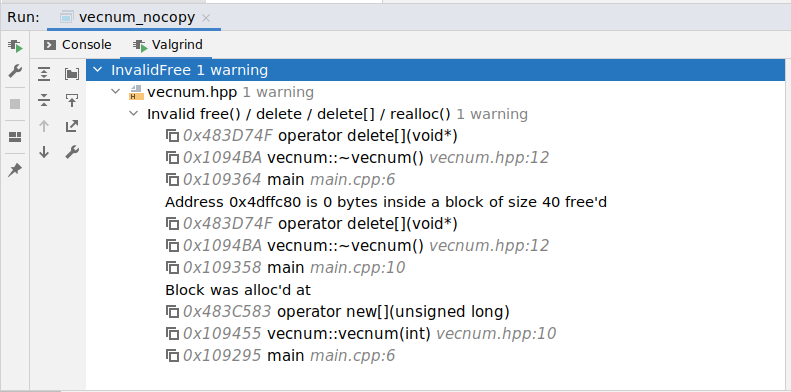
\includegraphics[width=\textwidth]{images/02-copia/vecnum-nocopy-valgrind.png}
\begin{itemize}
  \item Resultado similar con \textmark{Address Sanitizer}.
\end{itemize}
\end{frame}

\begin{frame}[t,fragile]{Copia y liberación}
\begin{itemize}
  \item \textbad{Problema}: Al realizar la copia, se ha copiado la dirección del array.
    \begin{itemize}
      \item Los dos vectores están compartiendo el mismo array.
      \item Se está desasignando dos veces un mismo bloque de memoria.
    \end{itemize}
\end{itemize}

\mode<presentation>{\vfill}
\begin{tikzpicture}
\tikzset{
    bloque/.style={rectangle,draw=black, top color=white, bottom color=blue!50,
                   very thick, inner sep=0.5em, minimum size=0.6cm, text centered, font=\tiny},
    flecha/.style={->, >=latex', shorten >=1pt, thick},
    etiqueta/.style={text centered, font=\tiny} 
}  
\node[bloque] (bsize) {5};
\node[bloque,right=0cm of bsize] (bptr) { };
\node[bloque,right=0.5cm of bptr] (v0) {0.0};
\node[bloque,right=0cm of v0] (v1) {0.0};
\node[bloque,right=0cm of v1] (v2) {5.0};
\node[bloque,right=0cm of v2] (v3) {0.0};
\node[bloque,right=0cm of v3] (v4) {3.5};
\draw[flecha] (bptr) -- (v0);
\node[etiqueta, left=0.1cm of bsize] {v1:};
\node[etiqueta, above=0cm of bsize] {tam};

\node[bloque, below=1cm of bsize] (bsize2) {5};
\node[bloque,right=0cm of bsize2] (bptr2) { };
\draw[flecha] (bptr2) -- (v0);
\node[etiqueta, left=0.1cm of bsize2] {v2:};

\end{tikzpicture}
\end{frame}

\section{Constructor de copia}

\begin{frame}[fragile]{Constructor de copia}
\begin{itemize}
  \item El \textgood{constructor de copia} se invoca cuando se 
        \textemph{construye un objeto} a partir de \textmark{otro del mismo tipo}.
    \begin{itemize}
      \item Toma un argumento referencia constante al tipo.
    \end{itemize}
\begin{lstlisting}
vecnum(const vector &);
\end{lstlisting}

  \mode<presentation>{\vfill\pause}
  \item Se puede suprimir la generación automática del constructor de copia.
\begin{lstlisting}
vecnum(const vecnum &) = delete;
\end{lstlisting}

  \mode<presentation>{\vfill\pause}
  \item El constructor de copia se invocará en definiciones del tipo:
\begin{lstlisting}
vecnum w {v}; // Iniciación directa
vecnum w(v);  // Iniciación directa. Sintaxis tradicional.
vecnum w = v; // Iniciación de copia. No es asignación.
\end{lstlisting}
\end{itemize}
\end{frame}

\begin{frame}[t]{Implementación de constructor de copia}
\begin{block}{vecnum.cpp}
\lstinputlisting[firstline=9,lastline=13]{ejemplos/02-copia/vecnum-copy/vecnum.cpp}
\end{block}

\mode<presentation>{\vfill}
\begin{enumerate}
  \item Copia el tamaño.
  \item Reserva memoria para un nuevo búfer.
  \item Copia los elementos del búfer origen en el búfer destino.
    \begin{itemize}
      \item \cppid{copy\_n(p,n,q)}: Copia \cppid{n} elementos consecutivos almancenados
            a partir de \cppid{p} en posiciones consecutivas a partir de \cppid{q}.
    \end{itemize} 
\end{enumerate}
\end{frame}

\section{Operador de asignación de copia}

\begin{frame}[t,fragile]{Operador de asignación de copia}
\begin{itemize}
  \item El \textgood{operador de asignación de copia} se invoca cuando
        \textemph{se asigna un objeto} a otro \textmark{del mismo tipo}.
    \begin{itemize}
      \item Toma un argumento referencia constante al tipo.
      \item Devuelve una referencia al objeto asignado.
      \item Debe ser una función miembro de la clase.
    \end{itemize}
\begin{lstlisting}
vecnum & operator=(const vecnum &);
\end{lstlisting}

  \mode<presentation>{\vfill\pause}
  \item Se puede suprimir la generación automática del operador de asignación de copia.
\begin{lstlisting}
vecnum & operator=(const vecnum &) = delete;
\end{lstlisting}

  \mode<presentation>{\vfill\pause}
  \item El constructor de copia se invocará en expresiones del tipo:
\begin{lstlisting}
w = v; // w.operator=(v);
\end{lstlisting}
\end{itemize}
\end{frame}

\begin{frame}[t,fragile]{Implementación de operador de asignación de copia}
\begin{block}{vector.cpp}
\begin{lstlisting}
vecnum & vecnum::operator=(const vecnum & v) {
  tamanyo_ = v.tamanyo_;
  delete []buffer_;
  buffer_ = new double[v.tamanyo_];
  std::copy_n(v.buffer_, v.tamanyo_, buffer_);
  return *this;
}
\end{lstlisting}
\end{block}

\mode<presentation>{\vfill}
\begin{itemize}
  \item Copiar el tamaño.
  \item Liberar el búffer anterior.
  \item Reservar un bloque de memoria para el nuevo búfer.
  \item Copiar elemento a elemento del buffer anterior al nuevo.
  \item Devolver una referencia al objeto acutal (\cppkey{*this}).
\end{itemize}
\end{frame}

\begin{frame}[t,fragile]{El puntero \textbf{this}}
\begin{itemize}
  \item \cppkey{this} es una palabra reservada que se puede evaluar
        \textmark{dentro} de cualquier \textgood{función miembro} de una clase.

  \mode<presentation>{\vfill\pause}
  \item Se evalúa a la \textmark{dirección de memoria} del objeto para el que se 
        está ejecutando la función miembro.
    \begin{itemize}
      \item \cppkey{this} es un puntero.
    \end{itemize}

  \mode<presentation>{\vfill\pause}
  \item La expresión \cppkey{return *this} en el operador de asignación de copia devuelve una referencia la objeto.

  \mode<presentation>{\vfill\pause}
  \item \textmark{¿Por qué?}
\begin{lstlisting}[escapechar=@]
v1 = v2 = v3; @\pause@
v1.operator=(v2=v3); @\pause@
v1.operator=(v.operator=(v3));
\end{lstlisting}
    \begin{itemize}
      \item Asociativo por la derecha.
    \end{itemize}
\end{itemize}
\end{frame}

\begin{frame}[t,fragile]{Optimizando la auto-asignación}
\begin{itemize}
  \item Caso particular: \textmark{auto-asignación}
\begin{lstlisting}
v = v; // v.operator=(v);
\end{lstlisting}
    \begin{itemize}
      \item Debería no hacerse nada.
    \end{itemize}

  \mode<presentation>{\vfill\pause}
\begin{block}{Constructor de copia}
\begin{lstlisting}
vecnum & vecnum::operator=(const vecnum & v) {
  if (this == &v) return *this;
  tamanyo_ = v.tamanyo_;
  delete []buffer_;
  buffer_ = new double[v.tamanyo_];
  std::copy_n(v.buffer_, v.tamanyo_, buffer_);
  return *this;
}
\end{lstlisting}
\end{block}
\end{itemize}
\end{frame}

\mode<article>{
  \section{Lecturas recomendadas}

\begin{enumerate}

\item .

\end{enumerate}

  \section{Ejercicios}

\begin{enumerate}

\item .

\end{enumerate}

}

\mode<article>{\chapter{\modulenoexcept}}

\mode<presentation>{\begin{frame}[shrink=20]{Licencia Creative Commons}

\begin{tabularx}{.98\textwidth}{lX}
\ccLogo & Este trabajo se distribuye bajo licencia
Atribución-NoComercial-SinDerivadas 4.0 Internacional (CC BY-NC-ND 4.0).\\

&\\

& \multicolumn{1}{c}{\textbf{Usted es libre de}:}\\

&\\

&
\textbf{Compartir} --
copiar y redistribuir el material en cualquier medio o formato.
\\

&\\

& \multicolumn{1}{c}{\textbf{Bajo los siguientes términos}:}\\

&\\

\ccAttribution &
Atribución -- Usted debe dar crédito de manera adecuada, brindar un enlace a la licencia, e indicar si se han realizado cambios. Puede hacerlo en cualquier forma razonable, pero no de forma tal que sugiera que usted o su uso tienen el apoyo de la licenciante.
\\

\ccNonCommercialEU &
NoComercial -- Usted no puede hacer uso del material con propósitos comerciales. 
\\

\ccNoDerivatives &
SinDerivadas -- Si remezcla, transforma o crea a partir del material, no podrá distribuir el material modificado. 
\\

\end{tabularx}

\end{frame}
}
\section{Propagación de excepciones}

\begin{frame}[t,fragile]{Propagación multinivel}
\begin{itemize}
  \item Una excepción se propaga a través de varios niveles hasta que alcanza
        un manejador que la captura.
\end{itemize}

\begin{columns}[T]

\column{.5\textwidth}
\mode<presentation>{\vfill\pause}
\begin{lstlisting}
void h(std::istream & is) {
  std::string s;
  is >> s;
  if (!valid(s)) throw formato_invalido{};
  //...
}

void g(const std::string & nombre) {
  std::ifstream entrada{nombre};
  h(entrada);
  //...
}
\end{lstlisting}

\column{.5\textwidth}
\mode<presentation>{\vfill\pause}
\begin{lstlisting}
void f(std::string & base) {
  std::string nombre = base + ".txt"
  try {
    g(nombre);
  }
  catch(formato_invalido) {
    // tratamiento del error
  }
}
\end{lstlisting}
\end{columns}

\mode<presentation>{\vfill\pause}
\begin{itemize}
  \item Permite separar el punto de detección del error del punto de tratamiento.
\end{itemize}
\end{frame}

\begin{frame}[t,fragile]{Objeto excepción}
\begin{itemize}
  \item Cuando se lanza una excepción de un tipo \cppid{E}:
\begin{lstlisting}
throw E;
\end{lstlisting}
    \begin{itemize}
      \item Se inicia un objeto temporal del tipo \cppid{E}.
      \item Se pasa el objeto temporal a la correspondiente claúsula \cppkey{catch}.
    \end{itemize}

  \mode<presentation>{\vfill\pause}
  \item El objeto excepción se puede potencialmente copiar una o varias vecces.
    \begin{itemize}
      \item Debe ser un objeto ligero (pocas palabras de memoria).
    \end{itemize}

  \mode<presentation>{\vfill\pause}
  \item La captura de la excepción puede ser:
    \begin{itemize}
      \item Por valor.
      \item Por referencia.
      \item Por referencia constante.
    \end{itemize}

\end{itemize}
\end{frame}

\begin{frame}[t,fragile]{Captura de excepciones por valor}
\begin{itemize}
  \item Se recibe una copia del objeto excepción.
\begin{lstlisting}[basicstyle=\tiny]
void f() {
  try {
    //...
  }
  catch(formato_invalido e) {
    std::cerr << e.mensaje() << "\n";
  }
}
\end{lstlisting}

  \mode<presentation>{\vfill\pause}
  \item Si no se necesita usar el objeto se puede omitir el nombre del parámetro.
\begin{lstlisting}[basicstyle=\tiny]
void f() {
  try {
    //...
  }
  catch(formato_invalido e) {
    std::cerr << e.mensaje() << "\n";
  }
}
\end{lstlisting}
\end{itemize}
\end{frame}

\begin{frame}[t,fragile]{Captura de excepciones por referencia}
\begin{itemize}
  \item Se puede capturar por referencia o referencia constante.
    \begin{itemize}
      \item Normalmente se prefiere referencia constante.
      \item Se recibe una referenica al objeto excepción.
    \end{itemize}
\begin{lstlisting}
void f() {
  try {
    //...
  }
  catch(const std::out_of_range & e) {
    //...
  }
  catch(const std::exception & e) {
    //...
  }
  catch(...) {
    //...
  }
}
\end{lstlisting}
\end{itemize}
\end{frame}

\begin{frame}[t,fragile]{Excepciones y destrucción}
\begin{itemize}
  \item Cuando se lanza una excepción se destruyen todos los objetos locales.
\begin{lstlisting}
void h(std::istream & is) {
  std::string s;
  is >> s;
  if (!es_valida(s)) throw formato_invalido{};
  //...
}
\end{lstlisting}
    \begin{itemize}
      \item Si la cadena \cppid{s} no \textmark{es valida}, al salir de
            la función se destruye el objeto local \cppid{s}.
    \end{itemize}
\end{itemize}
\end{frame}

\begin{frame}[t,fragile]{Desenrollado de pila}
\begin{itemize}
  \item Cuando se captura una excepción en un alcance, se transfiere el control
        desde el punto en el que se realiza el \cppkey{throw}.
    \begin{itemize}
      \item En cada alcance intermedio se produce el \textmark{desenrollado de
            la pila} (\emph{stack unwinding}).
      \item Se destruyen todos los objetos locales de cada alcance.
    \end{itemize}
\end{itemize}

\begin{columns}[T]

\column{.5\textwidth}
\mode<presentation>{\vfill\pause}
\begin{lstlisting}
void h(std::istream & is) {
  std::string s;
  is >> s;
  if (!valid(s)) throw formato_invalido{};
  //...
} // throw => destruir s

void g(const std::string & nombre) {
  std::ifstream entrada{nombre};
  h(entrada);
  //...
} // throw => destruir entrada
\end{lstlisting}

\column{.5\textwidth}
\mode<presentation>{\vfill\pause}
\begin{lstlisting}
void f(std::string & base) {
  std::string nombre = base + ".txt"
  try {
    g(nombre);
  } // throw => No se destruye nombre
  catch(formato_invalido) {
    // tratamiento del error
  }
}
\end{lstlisting}
\end{columns}

\end{frame}

\begin{frame}[t,fragile]{Excepciones no tratadas}
\mode<presentation>{\vspace{-0.75em}}
\begin{itemize}
  \item Si una excepción se propaga hasta el programa principal y tampo es tratada allí:
    \begin{itemize}
      \item Se invoca a la función \cppid{terminate()}.
      \item El \textgood{desenrollado de la pila} es 
            \textmark{dependiente de la implementación}.
    \end{itemize}
\end{itemize}

\mode<presentation>{\vspace{-0.5em}}
\pause
\begin{columns}[T]

\column{.5\textwidth}
\begin{block}{main.cpp}
\lstinputlisting[basicstyle=\tiny]{ejemplos/03-noexcept/escaping-exception/main.cpp}
\end{block}

\pause
\column{.5\textwidth}
\begin{lstlisting}[style=terminal]
terminate called after throwing an instance of 'error'

Process finished with exit code 134 (interrupted by signal 6: SIGABRT)
\end{lstlisting}

\end{columns}
\end{frame}

\begin{frame}[t]{Excepciones y destructores}
\begin{itemize}
  \item \textbad{No puede haber} más de una excepción en vuelo en un programa.
    \begin{itemize}
      \item Desde el punto de \cppkey{throw} hasta el punto de \cppkey{catch}
            \textbad{no se puede lanzar} otra excepción.
      \item Podría ocurrir si se destruye un objeto local y su destructor
            lanza una excepción.
      \item \textmark{Solución}: Evitar excepciones en destructores.
    \end{itemize}
\end{itemize}

\mode<presentation>{\vfill\pause}
\begin{columns}[T]

\column{.5\textwidth}
\lstinputlisting[lastline=9]{ejemplos/03-noexcept/double-exception/main.cpp}
\column{.5\textwidth}
\lstinputlisting[firstline=11]{ejemplos/03-noexcept/double-exception/main.cpp}

\end{columns}
\end{frame}

\begin{frame}[t]{Comportamiento de \textbf{terminate()}}
\mode<presentation>{\vspace{-0.5em}}
\begin{itemize}
  \item La función \cppid{std::terminate()} finaliza invocando a la función
        \cppid{std::abort()}.

  \mode<presentation>{\vfill\pause}
  \item Se puede instalar una función que se ejecute para tratar la terminación.

\mode<presentation>{\vspace{-0.5em}}
\begin{columns}[T]

\column{.6\textwidth}
\lstinputlisting{ejemplos/03-noexcept/terminate-handler/main.cpp}

\column{.4\textwidth}
\begin{itemize}
  \item Si la función de terminación no finaliza invocando a \cppid{std::abort()}
        la implementación invoca a \cppid{std::abort()}.
    \begin{itemize}
      \item \cppid{std::terminate()} \textbad{nunca} vuelve.
    \end{itemize}
\end{itemize}
\end{columns}

\end{itemize}
\end{frame}

\section{Garantías de excepciones}

\begin{frame}[t]{Invariantes y estado válido}
\begin{itemize}
  \item \textgood{Invariantes de clase}: Condiciones que comple un objeto
        establecidas por el \textmark{constructor} y mantenidas por todas las
        \textmark{operaciones} hasta la ejecución del \textmark{destructor}.

  \mode<presentation>{\vfill\pause}
  \item Tipo \cppid{vecnum}:
    \begin{itemize}
      \item \cppid{tamanyo\_ >= 0}.
      \item Si \cppid{tamanyo\_ == 0} $\Rightarrow$ \cppid{buffer\_ ==}\cppkey{nullptr}.
      \item Si \cppid{tamanyo\_ > 0} $\Rightarrow$ \cppid{buffer\_} apunta
            a un bloque de memoria dinámica capaz de albergar desde \cppid{buffer\_[0])}
            a \cppid{buffer\_[tamanyo\_-1]}.
    \end{itemize}

  \mode<presentation>{\vfill\pause}
  \item Un \textmark{objeto} se encuentra en un \textgood{estado válido} si:
    \begin{enumerate}
      \item Su constructor se ha ejecutado.
      \item Todas las operaciones ejecutadas mantienen las invariantes.
      \item Su destructor no se ha ejecutado.
    \end{enumerate}
\end{itemize}
\end{frame}

\begin{frame}[t]{Seguridad frente a excepciones}
\begin{itemize}
  \item Una \textmark{operación} es \textemph{segura frente a excepciones}
        (\emph{exception safe}) si la operación deja al programa en un 
        \textgood{estado válido} incluso cuando la operación 
        \textbad{termina lanzando una excepción}.

  \mode<presentation>{\vfill\pause}
  \item Cada operación debe ofrecer la \textemph{garantía mas estricta posible}
        de las siguientes:
    \begin{itemize}

      \mode<presentation>{\vfill\pause}
      \item \textgood{Garantía \emph{nothrow}} $\Rightarrow$ Algunas operaciones.
        \begin{itemize}
          \item La operación no lanza excepciones.
        \end{itemize}
      \mode<presentation>{\vfill\pause}

      \item \textgood{Garantía fuerte} $\Rightarrow$ Operaciones clave.
        \begin{itemize}
          \item La operación se completa o se deshacen los cambios.
        \end{itemize}

      \mode<presentation>{\vfill\pause}
      \item \textgood{Garantía básica} $\Rightarrow$ Todas las operaciones.
        \begin{itemize}
          \item Si hay error, el objeto puede seguir usándose.
        \end{itemize}
    \end{itemize}
\end{itemize}
\end{frame}

\begin{frame}[t,fragile]{Garantía básica}
\begin{itemize}
  \item La \textgood{garantía básica} requiere:
    \begin{itemize}
      \item Se mantienen las invariantes de todos los objetos.
      \item No hay goteo (pérdida) de ningún recurso.
    \end{itemize}

  \mode<presentation>{\vfill\pause}
  \item \textmark{Implicaciones}:
    \begin{itemize}
      \item El objeto puede destruirse.
      \item Se puede asignar otro valor a un objeto.
    \end{itemize}
\end{itemize}

\mode<presentation>{\vfill\pause}
\begin{lstlisting}
vecracional & vecracional::operator=(const vecracional & v) {
  tamanyo_ = v.tamanyo_;
  delete []buffer_;
  buffer_ = new racional[tamanyo_]; // bad_alloc, racional()
  for (int i=0; i<tamanyo_; ++i) {
    buffer_[i] = v.buffer_[i]; // operator=
  }
  return *this;
}
\end{lstlisting}
\end{frame}

\begin{frame}[t,fragile]{Cumpliendo la garantía básica}
\begin{itemize}
  \item \textmark{Razones} para fallo de la sentencia:
\begin{lstlisting}
buffer_ = new racional[tamanyo_];
\end{lstlisting}
    \begin{itemize}
      \item Excepción \cppid{std::bad\_alloc}: No queda memoria.
      \item Alguna excepción lanzada por constructor de \cppid{racional}.
    \end{itemize}

  \mode<presentation>{\vfill\pause}
  \item \textmark{Efectos}:
    \begin{itemize}
      \item \cppid{buffer\_} quedaría apuntando a memoria liberada.
      \item \textbad{No se puede} ejecutar el \textgood{destructor}.
    \end{itemize}
\end{itemize}

\mode<presentation>{\vfill\pause}
\begin{lstlisting}
vecracional & vecracional::operator=(const vecracional & v) {
  auto aux = new racional[v.tamanyo_]; // bad_alloc, racional()
  tamanyo_ = v.tamanyo_;
  delete []buffer_;
  buffer_ = aux;
  for (int i=0; i<tamanyo_; ++i) {
    buffer_[i] = v.buffer_[i]; // operator=
  }
  return *this;
}
\end{lstlisting}
\end{frame}

\begin{frame}[t,fragile]{Garantía fuerte}
\begin{itemize}
  \item La \textmark{garantía fuerte} requiere:
    \begin{itemize}
      \item Cumplir la garantía básica, y además,
      \item O la operación tiene éxito o no tiene efecto.
    \end{itemize}

  \mode<presentation>{\vfill\pause}
  \item \textmark{Consecuencias}:
    \begin{itemize}
      \item Ejecutar todas las operaciones que podrían fallar antes de empezar 
            a modificar el estado del objeto.
    \end{itemize}
\end{itemize}

\mode<presentation>{\vfill\pause}
\begin{lstlisting}
vecracional & vecracional::operator=(const vecracional & v) {
  auto aux = new racional[v.tamanyo_]; // bad_alloc, racional()
  std::copy_n(v.buffer_, v.tamanyo_, aux); // operator=
  tamanyo_ = v.tamanyo_;
  delete []buffer_;
  buffer_ = aux;
  return *this;
}
\end{lstlisting}
\end{frame}

\begin{frame}[t,fragile]{Garantía \textbf{nothrow}}
\begin{itemize}
  \item La \textmark{garantía \emph{nothrow}} requiere:
    \begin{itemize}
      \item Cumplir la garantía fuerte, y además,
      \item No lanzar ninguna excepción.
    \end{itemize}
\end{itemize}

\mode<presentation>{\vfill\pause}
\begin{lstlisting}[basicstyle=\tiny,escapechar=@]
class vecracional {
public:
  //...
  const & racional operator[](int i) const { // Garantía nothrow
    return buffer_[i];
  }

  racional & operator[](int i) { // Garantía nothrow
    return buffer_[i];
  }
  @\pause@
  const racional & posicion(int i) const { // Garantía fuerte
    if (i<0 || i>=tamanyo_) throw std::range_error{"racional::posicion()"};
    return buffer_[i];
  }

  racional & posicion(int i) { // Garantía fuerte
    if (i<0 || i>=tamanyo_) throw std::range_error{"racional::posicion()"};
    return buffer_[i];
  }
  //...
};
\end{lstlisting}
\end{frame}

\section{Especificiaciones de excepciones}

\begin{frame}[t,fragile]{Funciones que lanzan excepciones}
\begin{itemize}
  \item Normalmente, una función, puede lanzar una excepción.
\begin{lstlisting}
void suma(int x, int y); // Puede lanzar excepciones
\end{lstlisting}

  \mode<presentation>{\vfill\pause}
  \item Se puede utilizar la especificación \cppkey{noexcept} para
        indicar que una función \textmark{ofrece la garantía \emph{noexcept}}.
\begin{lstlisting}
void suma(int x, int y) noexcept; // No lanza excepciones
\end{lstlisting}

  \mode<presentation>{\vfill\pause}
  \item La claúsula \cppkey{noexcept} acepta un argument booleano.
\begin{lstlisting}
void suma(int x, int y) noexcept(true); // No lanza excepciones
void suma(int x, int y) noexcept(false); // Puede lanzar excepciones
\end{lstlisting}


  \mode<presentation>{\vfill\pause}
  \item \textbad{No se comprueba} en tiempo de compilación 
        si la especificación es cierta.
    \begin{itemize}
      \item Requeriría análisis completo de programa durante la fase de enlace.
    \end{itemize}
\end{itemize}
\end{frame}

\begin{frame}[t,fragile]{Violación de especificación de excepciones}
\begin{itemize}
  \item Si una función marcada con \cppkey{noexcept} acaba lanzando una
        excepción, se ha producido una \textbad{violación de especificación noexcept}.

  \mode<presentation>{\vfill\pause}
  \item \textgood{Efecto}:
    \begin{itemize}
      \item El programa \textmark{termina su ejecución} invocando a \cppid{std::terminate()}.
      \item \textbad{No hay garantía} de que se ejecuten los destructores desde el punto
            de \cppkey{throw} al punto de \cppkey{noexcept}.
      \item \textbad{No hay garantía} de 
            \textmark{desenrollado de la pila} (\emph{stack unwinding}).
      \item \textbad{No hay posibilidad} de \textmark{recuperarse} y 
            \textmark{continuar} la ejecución del programa.
    \end{itemize}

  \mode<presentation>{\vfill\pause}
  \item Cuando se marca una función como \cppid{noexcept} se está indicando
        que esta función \textmark{no propaga excepciones}.
\end{itemize}
\end{frame}

\begin{frame}[t,fragile]{Garantía \emph{nothrow}}
\begin{itemize}
  \item La \textmark{garantía \emph{nothrow}} es más difícil de obtener
        de lo que puede parecer.

\mode<presentation>{\vfill\pause}
\begin{lstlisting}[escapechar=@]
void cubo(int x) noexcept {
  return x*x*x;
}

std::vector<int> cubo(const std::vector<int> & v) @{\color{red}noexcept@ {
  std::vector<int> resultado(v.size()); // Podría lanzar std::bad_alloc
  for (std::size_t i=0; i<v.size(); ++i) {
    r.at(i) = cubo(v.at(i)); // Podría lanzar std::out_of_range?
  }
  return r;
}
\end{lstlisting}

  \mode<presentation>{\vfill\pause}
  \item Cualquier operación que implique reserva de memoria podría 
        \textmark{potencialmente} \textbad{lanzar una excepción}
        \cppid{std::bad\_alloc}.

  \mode<presentation>{\vfill\pause}
  \item A veces se puede deducir del contexto que una función 
        \textgood{no lanzará excepciones}.

\end{itemize}
\end{frame}

\begin{frame}[t,fragile]{Operador \emph{noexcept}}
\begin{itemize}
  \item La palabra reservada \cppkey{noexcept} se puede usar como un operador
        sobre una expresión.
    \begin{itemize}
      \item Se puede aplicar a cualquier expresión.
      \item Produce un resultado \textemph{booleano}.
      \item Indica si la evaluación de la expresión es \cppkey{noexcept}.
    \end{itemize}
\begin{lstlisting}
constexpr bool cond = noexcept(v.at(0));
\end{lstlisting}

  \mode<presentation>{\vfill\pause}
  \item Se puede usar para expresar la condición \cppkey{noexcept} de una función.
\begin{lstlisting}
void f(std::vector<double> & v) noexcept(noexcept(v.at(0)));
\end{lstlisting}

  \mode<presentation>{\vfill\pause}
  \item \textmark{Evaluación}:
    \begin{itemize}
      \item La expresión se evalúa en tiempo de compilación solamente.
      \item Se comprueba si las subexpresiones están marcadas como \cppkey{noexcept}.
    \end{itemize}

\end{itemize}
\end{frame}

\begin{frame}[t,fragile]{Excepciones y destructores}
\begin{itemize}
  \item En general, un destructor \textbad{no debería lanzar excepciones}.
    \begin{itemize}
      \item Los destructores de la biblioteca estándar son \cppkey{noexcept}.
      \item El destructor para un tipo es, por defecto, \cppkey{noexcept}
            si todos los miembros del tipo tienen destructores \cppkey{noexcept}.
    \end{itemize}

\mode<presentation>{\vfill}
\begin{lstlisting}
class estudiante {
public:
  //...
  ~estudiante(); // Implícitamente noexcept
private:
  std::string nombre;
  std::vector<std::string> calificaciones;
};
\end{lstlisting}
\end{itemize}
\end{frame}

\mode<article>{
  \section{Lecturas recomendadas}

\begin{enumerate}

\item .

\end{enumerate}

  \section{Ejercicios}

\begin{enumerate}

\item .

\end{enumerate}

}



\nocite{*}
\bibliographystyle{abbrv}
\bibliography{bib/cppref}

\end{document}
